\documentclass[border=8pt]{standalone}
\usepackage[T1]{fontenc}
\usepackage{times}
\usepackage{amsmath,amssymb}
\usepackage{xcolor}
\usepackage{tikz}
\usetikzlibrary{arrows.meta,positioning,calc}
\begin{document}
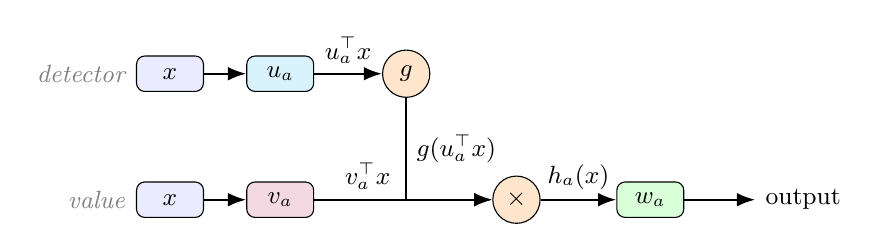
\begin{tikzpicture}[
    >=Latex,
    every node/.style={font=\small},
    box/.style={draw, rounded corners=3pt, minimum width=0.85cm,
                minimum height=0.45cm, inner sep=2pt},
    op/.style={draw, circle, minimum size=0.6cm, inner sep=0pt},
    arr/.style={->, thick, >=Latex},
    rolelabel/.style={font=\small\itshape, text=gray}
]

    \node[box, fill=blue!8]   (x1) at (-3.4,  0.8) {$x$};
    \node[box, fill=blue!8]   (x2) at (-3.4, -0.8) {$x$};

    \node[box, fill=cyan!15]  (u)  at (-2.0,  0.8) {$u_a$};
    \node[box, fill=purple!15](v)  at (-2.0, -0.8) {$v_a$};

    \node[op,  fill=orange!20] (g)   at (-0.4,  0.8) {$g$};
    \node[op,  fill=orange!20] (mul) at ( 1, -0.8) {$\times$};

    \node[box, fill=green!15] (w)   at ( 2.7, -0.8) {$w_a$};

    \node[rolelabel, anchor=east] at (-3.85,  0.8) {detector};
    \node[rolelabel, anchor=east] at (-3.85, -0.8) {value};

    \draw[arr] (x1) -- (u);
    \draw[arr] (u) -- node[above]{$u_a^\top x$} (g);
    \draw[arr] (g.south) -- node[right]{$g(u_a^\top x)$}
                         (g.south |- mul.west) -- (mul.west);

    \draw[arr] (x2) -- (v);
    \draw[arr] (v.east) -- node[above, pos=0.3]{$v_a^\top x$} (mul);

    \draw[arr] (mul) -- node[above]{$h_a(x)$} (w);
    \draw[arr] (w.east) -- ++(0.9, 0) node[right]{output};
\end{tikzpicture}
\end{document}
